\section{Drawbacks of Existing Methods for mVAM Data}

The nature of the mVAM data precluded any pre-existing methods for RCS data from being ideal. The lack of macro-level variables changing over time meant that the approach proposed by ----- wan't viable. The consistency in rates of assistance and displacement in daily samples meant that the effects of such factors would be obfuscated by calculating daily aggregates and fitting a time series with covariates. In order to fit such a model, individual-level variables such as \textit{Assistance} and \textit{Displacement} would have to be used to generate daily aggregates, namely the proportion of the daily sample that is receiving aid or has displaced household members. However, should sampling be designed to maintain a relatively constant proportion each day, then there is no variance to allow for an effect to be captured. Let's generate a simple version of such a model. The method most befitting was proposed by Modugno, in which temporal correlation is modeled by the addition of a latent time series to a standard fixed effects model.

Let's look at the implications of treating a dataset with daily and individual variance as a time series with covariates. 

\begin{figure}[H]
    \centering
    
    \begin{subfigure}{0.48\textwidth}
        \centering
        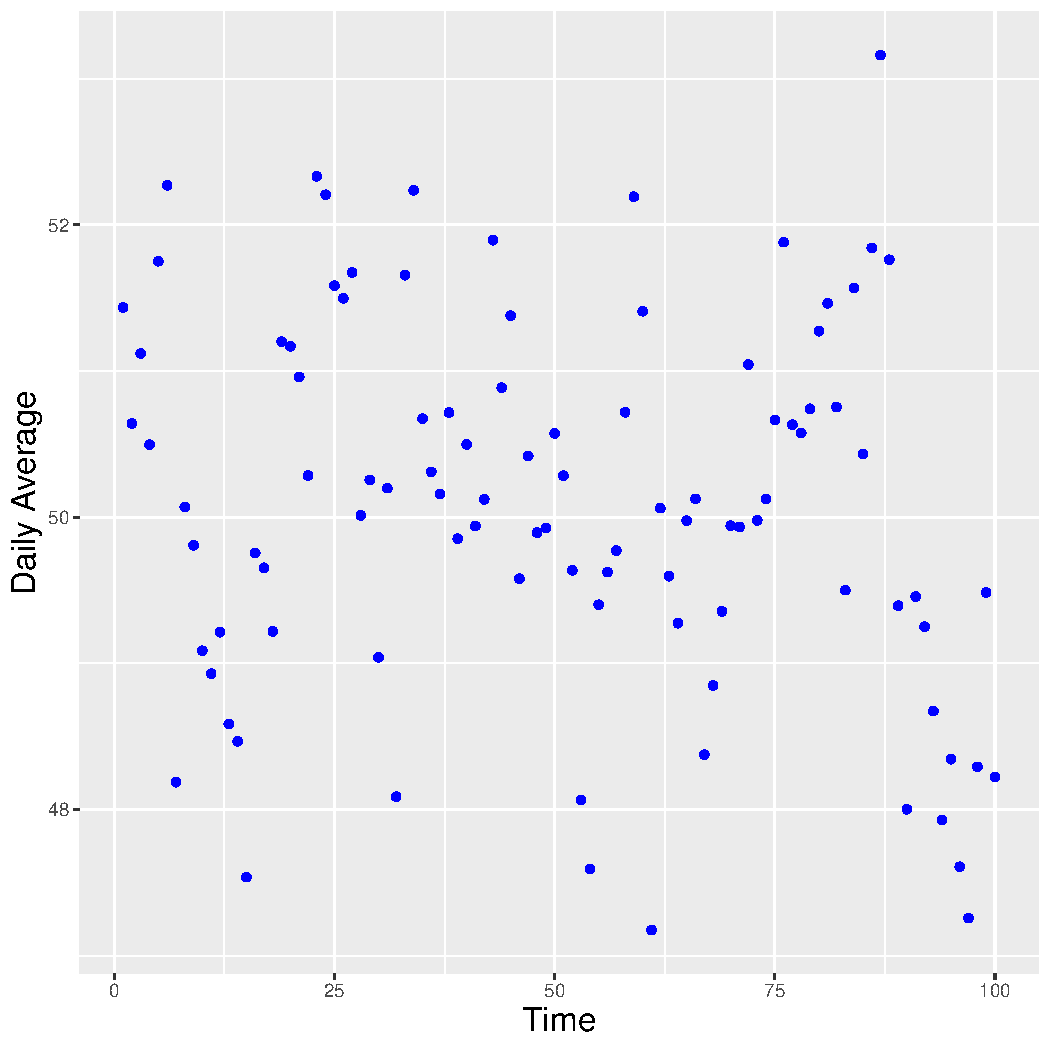
\includegraphics[width=\linewidth]{images/output/avg_y.pdf}
        \caption{Averages of simulated data with fixed effects and latent time series}
    \end{subfigure}
    \hfill
    \begin{subfigure}{0.48\textwidth}
        \centering
        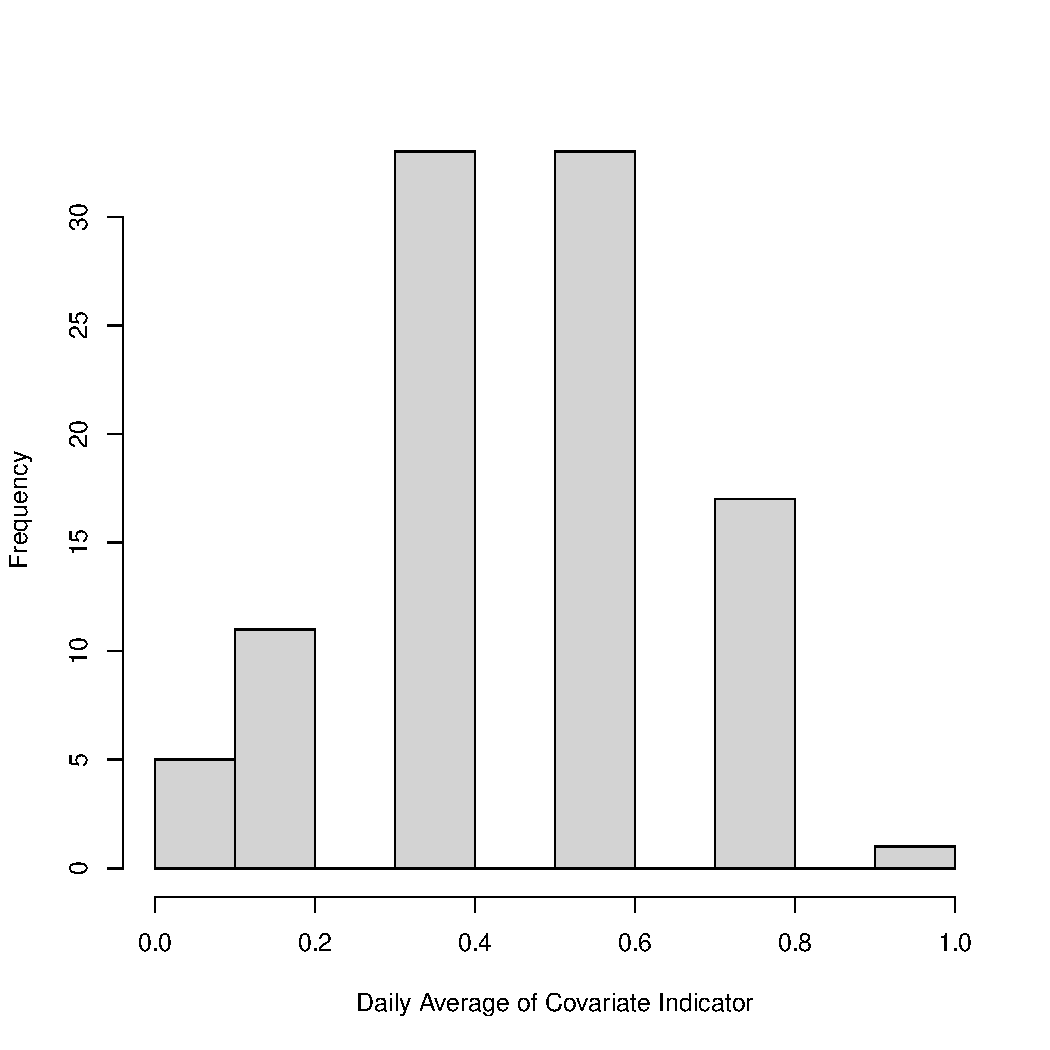
\includegraphics[width=\linewidth]{images/output/xreghist.pdf}
        \caption{Histogram of daily averages for binary covariate}
    \end{subfigure}
    \caption{Sample Noise and Corresponding Sample Sizes}
\end{figure}

If the true model is defined by $\yy = X_f\beta + x_t\uu + \varepsilon$, in which $T = 1000$, $\{n_t\} \overset{\text{i.i.d}}{\sim} \text{Poi}(100)$, $\beta = (43,-0.001,0.25)'$, $\phi = .5$, $\theta = .5$, $\sigma_\varepsilon^2 = 100$, $\sigma_\eta^2 = 1$. The indicator variable $X_{ti}$ for the dummy fixed effect covariate is a vector of independent Bernouli variables with probability $0.5$. 

The daily averages are then modeled by:

\begin{equation}
    \label{armanem_averaged1}
    N^{-1}X_t'\yy = N^{-1}X_t'(X_f\beta + \uu + \varepsilon)
\end{equation}

\begin{equation}
    \label{armanem_averaged2}
    \bar{\yy} = X_f^*\beta + \uu + \mathbf{a}
\end{equation}

What we now get is a vector of daily averages in which $\bar{\yy}_t = 43 -.001t + \bar{\mathbf{x}}_t + u_t + a_t $

If we fit an ARMA model with covariates to this data set, we get the following results (based on 100 independent simulations):

\input{images/output/arma_cov_df.txt}

 
Note that the estimate mean for $\theta$ appears to be heavily biased. The truth is that the empirical mean's vicinity to 0 is no accident, but rather the product of a very specific set of circumstances regarding the other parameters. This change will be explained in greater detail later on, but for now it will suffice to say that the time series being fit is the sum of the original time series and the daily averages of individual noise hence the seemingly overestimated time series parameter.

Of greater concern is the fact that fixed effect parameters such as the dummy covariate categorically underperform. Even though there was some variance in the daily proportions of subjects belonging to the control group, the overal consistency of said proportions prevented the effect of the covariate from being modeled. In the very plausible scenario that sampling aims to maintain consistent proportions across groups, the aggregation necessary for fitting a time series with covariates results in too much information loss at the individual level. As such, we turn to a method (\citep{modugno2015multilevel})that models temporal correlation without the presence of macro-level variables or collapsing the two forms of variance.